\section{Secondary quantization}
	
	\subsection{Introduction}
	
	Second quantization starts with an expansion of a scalar or vector field (or wave functions) in a basis consisting of a complete set of functions. These expansion functions depend on the coordinates of a single particle. The expansion coefficients have been promoted from ordinary numbers to operators, creation and annihilation operators. A creation operator creates a particle in the corresponding basis function and an annihilation operator annihilates a particle in this function.
	
	
	\subsection{System for $\vec{A}$}
	
	Let us write Maxwell equations in vacuum without any charge in the system (in CGS units):
	\begin{numcases}{}
		\Rot \vec{E} = - \frac{1}{c} \parder{\vec{H}}{t},
		\label{eq:M1} \\
		\Rot \vec{H} = \frac{1}{c} \parder{\vec{E}}{t},
		\label{eq:M2} \\
		\Div \vec{E} = 0,
		\label{eq:M3} \\
		\Div \vec{H} = 0.
		\label{eq:M4}
	\end{numcases}
	It's more convenient to work with potentials but not the fields itself. If we know $\vec{A}$ и $\varphi$, we know the field
	\begin{eqnarray}
		\vec{E} &=& - \frac{1}{c} \parder{\vec{A}}{t} - \nabla \varphi, \label{eq:E_field}\\
		\vec{H} &=& \Rot \vec{A}.
	\end{eqnarray}
	It's easy to construct two (generally speaking infinitely many) different potential which can lead to the same EM fields. So we can put one arbitrary condition for $\vec{A}$ and $\varphi$. Let us use Lorentz gauge:
	\begin{equation}
		\Div \vec{A} = 0.
		\label{eq:Lorentz}
	\end{equation}
	
	Let us obtain an equation for $\vec{A}$. Substitution of field to the \eqref{eq:M2} gives us
	\begin{equation}
		\Rot \Rot \vec{A} = - \frac{1}{c^2} \parder{^2 \vec{A}}{t^2} - \frac{1}{c} \nabla \parder{\varphi}{t}
	\end{equation}
	and since
	\begin{equation}
		\Rot \Rot \vec{A} = \underbrace{\Grad \Div \vec{A}}_{\hookrightarrow = 0} - \Div \Grad \vec{A} = - \Delta \vec{A}
	\end{equation}
	then
	\begin{equation}
		\Delta \vec{A} - \frac{1}{c^2} \parder{^2 \vec{A}}{t^2} = \frac{1}{c} \nabla \parder{\varphi}{t}.
		\label{eq:temp1}
	\end{equation}
	If we do $\nabla\cdot$\eqref{eq:E_field} then we get
	\begin{equation}
		\underbrace{\Div \vec{E}}_{\hookrightarrow=0} = - \underbrace{\frac{1}{c} \parder{}{t} \Div \vec{A}}_{\hookrightarrow=0} - \Delta \varphi \quad \to \quad \Delta \varphi = 0 \quad \to \quad \nabla \varphi = 0.
	\end{equation}
	So we have system for $\vec{A}$:
	\begin{equation}
		\begin{cases}
			\Delta \vec{A} - \dfrac{1}{c^2} \parder{^2 \vec{A}}{t^2} = 0, \\ \\
			\Div \vec{A} = 0.
		\end{cases}
		\label{eq:forA}
	\end{equation}
	\textit{Remark:} in deriving this system we put $\rho = 0$ and $\vec{j} = 0$.
	
	\subsection{Formulation of the problem}
	
	Let us consider a cube with length of the edge $L$ (fig \ref{fig:cube}). Boundary conditions \textcolor{red}{should be zero or periodic} with the period $L$. System is considered to be conservative. The main idea is to solve system \eqref{eq:forA} and then just find the limit $L \to \infty$.
	
	\begin{figure}
		\centering
		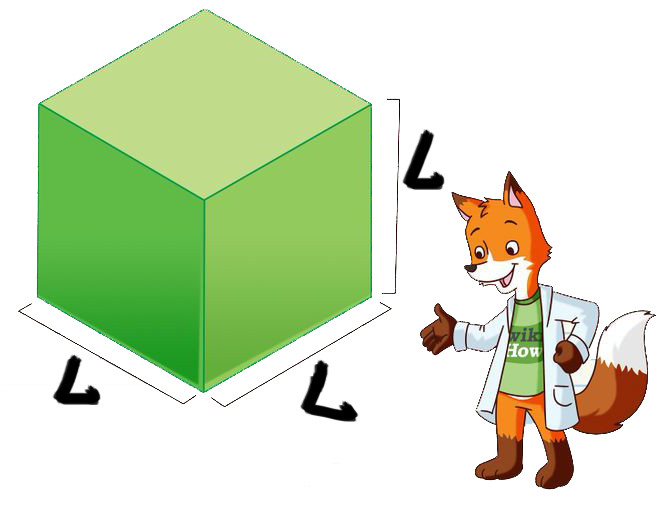
\includegraphics[width=0.5\linewidth]{fig/L1/cube}
		\caption{Formulation of the problem}
		\label{fig:cube}
	\end{figure}

	Solution of \eqref{eq:forA} may be written as the sum of all eigen solutions (each of it is a plane wave) in respect that boundary conditions are periodic:
	\begin{equation}
		\vec{A}(\vec{r},t) = \sum_{\vec{k}} \vec{A}_{\vec{k}}(t) e^{i \vec{k} \vec{r}}, \qquad k_{\alpha} = \frac{2 \pi n_{\alpha}}{L}, \quad \alpha = x,y,z.
	\end{equation}
	%Where $\vec{n}$ --- a unit vector. 
\textcolor{red}{Where $n_{\alpha}$ --- is an integer number.}
As waves are plane then we should write
	\begin{equation}
		\vec{A}_{\vec{k}}(t) = \vec{c}_{\vec{k}} e^{-i \omega_{\vec{k}}t} + \vec{c}_{-\vec{k}}^* e^{i \omega_{\vec{k}}t},
	\end{equation}
	where $\omega_{\vec{k}} = c k = c\sqrt{k_x^2 + k_y^2 + k_z^2}$. 
Let us make a remark: $\vec{A}_{\vec{k}} \in \mathbb{R}$, \textcolor{red}{so
\begin{equation}\label{kminsk}
		\vec{A}_{\vec{k}}(t)=\vec{A}_{\vec{k}}^*(t) = \vec{c}_{-\vec{k}} e^{-i \omega_{\vec{k}}t}+ \vec{c}_{\vec{k}}^* e^{i \omega_{\vec{k}}t}=\vec{A}_{\vec{-k}}(t),
	\end{equation} }.
	The Lorentz gauge leads to the fact that \textit{waves are transverse}:
	\begin{equation}
		\Div \vec{A} = 0 \quad \to \quad \sum \vec{k} \vec{A}_{\vec{k}} e^{i \vec{k} \vec{r}} = 0 \quad \Longleftrightarrow \quad \boxed{\vec{A}_{\vec{k}}(t) \cdot \vec{k} = 0.}
	\end{equation} 
	
	Consider a wave with wave vector $\vec{k}$. According to Maxwell equations, there are two independent polarizations, so we introduce two transverse polarization vectors $\vec{e}_{\vec{k}1}; \vec{e}_{\vec{k}2}$. Three vectors $(\vec{e}_{\vec{k}1}; \vec{e}_{\vec{k}2}; \vec{k}/k)$ form a right-handed orthonormal basis which implies:
	\begin{equation}
		\begin{matrix}
			\vec{k} \cdot \vec{e}_{\vec{k}s} = 0, && \vecmult{\vec{e}_{\vec{k}1}}{\vec{e}_{\vec{k}2}} = \vec{k}/k, \\ \\
			\vec{e}_{\vec{k}s} \cdot \vec{e}_{\vec{k}s'} = \delta_{ss'}, && \vec{c}_{\vec{k}} = \sum_s c_{\vec{k}s} \vec{e}_{\vec{k}s}.
		\end{matrix}
	\end{equation}
	After that we can rewrite decomposition of $\vec{A}$ as
	\begin{multline}
		\vec{A} = \sum_{\vec{k},s} \tilde{A}_{\vec{k}} \left( c_{\vec{k}s} \vec{e}_{\vec{k}s} e^{-i \omega_{\vec{k}} t} + c^*_{-\vec{k}s} \vec{e}^*_{-\vec{k}s}  e^{i \omega_{\vec{k}} t} \right) \cdot e^{i \vec{k} \vec{r}} = \\
		= \left/ \text{inverse 2nd sum \textcolor{red}{using \eqref{kminsk}}: } (-k) \to k \right/ =\sum_{\vec{k},s} \tilde{A}_{\vec{k}} \left( u_{\vec{k}s}(t) \vec{e}_{\vec{k}s} e^{i \vec{k} \vec{r}} + u^*_{\vec{k}s}(t) \vec{e}^*_{\vec{k}s}  e^{-i \vec{k} \vec{r}} \right),
	\end{multline}
	where $u_{\vec{k}s}(t) = c_{\vec{k}s} e^{-i \omega_{\vec{k}} t}$. Now we can write fields
	\begin{equation}
		\vec{E} = -\frac{1}{c} \parder{\vec{A}}{t} = \frac{i}{c} \sum_{\vec{k},s} \tilde{A}_{\vec{k}} \omega_{\vec{k}} \left( u_{\vec{k}s}(t) \vec{e}_{\vec{k}s} e^{i \vec{k} \vec{r}} - u^*_{\vec{k}s}(t) \vec{e}^*_{\vec{k}s}  e^{-i \vec{k} \vec{r}} \right),
	\end{equation}
	\begin{equation}
		\vec{H} = \Rot \vec{A} = i \sum_{\vec{k},s} \tilde{A}_{\vec{k}} \left( u_{\vec{k}s} \left[ \vec{k} \times \vec{e}_{\vec{k}s} \right] e^{i \vec{k} \vec{r}} - u^*_{\vec{k}s} \left[ \vec{k} \times \vec{e}^*_{\vec{k}s} \right] e^{-i \vec{k} \vec{r}} \right).
	\end{equation}
	
	The energy of EM field
	\begin{equation}
		\mathscr{H} = \frac{1}{8 \pi} \int \left(\vec{H}^2 + \vec{E}^2 \right) dV.
	\end{equation} 
	\textit{Remark:} there is no averaging over time!
	
	To make next calculations easier, let us notice that
	\begin{eqnarray}
		\int \limits_{L^3} e^{i (\vec{k} - \vec{k}')\vec{r}} dV = L^3 \delta_{\vec{k}\vec{k}'}.
	\end{eqnarray}
	This feature vanish the $\sum_{\vec{k}}$. Besides, it's convenient to notice that
	\begin{equation}
		\vec{e}_{\vec{k}s}^* \cdot \vec{e}_{\vec{k}s'} = \delta_{ss'} \qquad \to \qquad
		\left[ \vec{k} \times \vec{e}_{\vec{k}s}^* \right] \cdot \left[ \vec{k} \times \vec{e}_{\vec{k}s'} \right] = k^2 \delta_{ss'}.
	\end{equation}
	Then we get
	\begin{equation}
		\mathscr{H} = \frac{L^3}{8 \pi}\textcolor{red}{2} \sum_{\vec{k},s} \tilde{A}_{\vec{k}}^2 \Bigg( \underbrace{\frac{\omega_{\vec{k}}^2}{c^2} \left| u_{\vec{k}s} \right|^2}_{\hookrightarrow E^2} + \underbrace{k^2 \left| u_{\vec{k}s} \right|^2}_{\hookrightarrow H^2}  \Bigg), \qquad k^2 = \frac{\omega_{\vec{k}}^2}{c^2} \text{\ \ (for each mode!)}
	\end{equation}
	\begin{equation}
		\mathscr{H} = \frac{L^3}{\textcolor{red}{2} \pi} \sum_{\vec{k},s} \tilde{A}_{\vec{k}}^2 k^2 \left| u_{\vec{k}s} \right|^2.
	\end{equation}
	Segregation if real and imaginary part of mode can be done by introducing new variables
	\begin{eqnarray}
		q_{\vec{k}s}(t) &=& u_{\vec{k}s}(t) + u^*_{\vec{k}s}(t) , \\
		p_{\vec{k}s}(t) &=& -i \omega_{\vec{k}}  \left( u_{\vec{k}s}(t) - u^*_{\vec{k}s}(t) \right).
	\end{eqnarray}
	It's obvious that
	\begin{equation}
		u_{\vec{k}s}(t) = \frac{1}{2} q_{\vec{k}s}(t) - \frac{1}{2 i \omega} p_{\vec{k}s}(t) \quad \to \quad \left| u_{\vec{k}s} \right|^2 = \frac{1}{4 \omega_{\vec{k}}^2} \left( p^2_{\vec{k}s} + \omega^2_{\vec{k}} q_{\vec{k}s}^2 \right).
	\end{equation}
	The Hamiltonian function will be as follows
	\begin{equation}
		\mathscr{H} = \frac{L^3}{\textcolor{red}{4} \pi c} \sum_{\vec{k},s} \frac{\tilde{A}_{\vec{k}}^2}{2} \left( p^2_{\vec{k}s} + \omega^2_{\vec{k}} q_{\vec{k}s}^2 \right).
	\end{equation}
	Let us boldly put $\tilde{A}_{\vec{k}} = \sqrt{\textcolor{red}{4} \pi c^2/L^3}$, then finally
	\begin{equation}
		\mathscr{H} = \sum_{\vec{k},s}  \left( \frac{p^2_{\vec{k}s}}{2}+ \frac{\omega^2_{\vec{k}} q_{\vec{k}s}^2}{2} \right).
	\end{equation}
	
	If we can write full energy of the system like $\mathscr{H} \sim p^2/2 + \omega^2 q^2/2$, then it means this system can be quantize.  So next, we  \textit{quantize fields}. First of all we need to move to operators by doing
	\begin{equation}
		\begin{cases}
		q_{\vec{k}s} \to \hat{q}_{\vec{k}s}, \\
		p_{\vec{k}s} \to \hat{p}_{\vec{k}s}.
		\end{cases}
	\end{equation}
	After that our Hamiltonian function will transform to Mr. Hamiltonian. 
	Besides, coordinate and impulse operator must obey next commutation relations:
	\begin{equation}
		\left[\hat{q}_{\vec{k}s} ; \hat{p}_{\vec{k}'s'} \right] = i \hbar \delta^{(3)}_{\vec{k}\vec{k}'} \delta_{ss'},
		\label{eq:con1}
	\end{equation} 
	\begin{equation}
		\left[\hat{q}_{\vec{k}s} ; \hat{q}_{\vec{k}'s'} \right] = \left[\hat{p}_{\vec{k}s} ; \hat{p}_{\vec{k}'s'} \right] = 0.
		\label{eq:con2}
	\end{equation}
	Moreover, this operators must be Hermitian because $\mathscr{H}$ stands for real energy which we can measure. Therefore
	\begin{equation}
		\hat{q}_{\vec{k}s} = \hat{q}^{\dagger}_{\vec{k}s}, \qquad \hat{p}_{\vec{k}s} = \hat{p}^{\dagger}_{\vec{k}s}.
		\label{eq:con3}
	\end{equation}
	Relations \eqref{eq:con1}, \eqref{eq:con2} and \eqref{eq:con3} impose conditions for $\hat{q}_{\vec{k}s}$ and $\hat{p}_{\vec{k}s}$.
	Hereafter we can introduce ladder operators:
	\begin{eqnarray}
		\hat{a}_{\vec{k}s}(t) &=& \dfrac{1}{\sqrt{2 \hbar \omega}} \left( \omega \hat{q}_{\vec{k}s} + i \hat{p}_{\vec{k}s} \right), \\ \nonumber \\
		\hat{a}^{\dagger}_{\vec{k}s}(t) &=& \dfrac{1}{\sqrt{2 \hbar \omega}} \left( \omega \hat{q}_{\vec{k}s} - i \hat{p}_{\vec{k}s} \right).
	\end{eqnarray}
	This leads to the useful representation of $\hat{q}_{\vec{k}s}$ and $\hat{p}_{\vec{k}s}$:
	\begin{eqnarray}
		\hat{q}_{\vec{k}s}(t) &=& \sqrt{\dfrac{\hbar}{2 \omega}} \left( \hat{a}^{\dagger}_{\vec{k}s} +  \hat{a}_{\vec{k}s} \right), \\ \nonumber \\
		\hat{p}_{\vec{k}s}(t) &=& i \sqrt{\dfrac{\hbar \omega}{2}} \left( \hat{a}^{\dagger}_{\vec{k}s} -  \hat{a}_{\vec{k}s} \right).
	\end{eqnarray}
	
	Commutation relations can be easily derived from consideration $\left[ \hat{q}_{\vec{k}s} ; \hat{p}_{\vec{k}s} \right]$ in the repre-sentation  of ladder operators and using \eqref{eq:con1} and \eqref{eq:con2}. So we get
	\begin{equation}
		\left[ \hat{a}_{\vec{k},s} ; \hat{a}^{\dagger}_{\vec{k}',s'} \right] = \delta^{(3)}_{\vec{k}\vec{k}'} \delta_{ss'}.
	\end{equation}
	
	Easy to show that Hamiltonian can be written as follows
	\begin{equation}
		\hat{\mathscr{H}} = \sum_{\vec{k},s} \hbar \omega_{\vec{k}} \left[ \hat{a}^{\dagger}_{\vec{k},s} \hat{a}_{\vec{k},s} + \frac{1}{2} \right].
	\end{equation}
	